\chapter{Tools for reproducible robotics}\label{ch:ducker}

\setlength{\epigraphwidth}{0.73\textwidth}
\epigraph{``An article about computational science in a scientific publication is not the scholarship itself, it is merely advertising of the scholarship. The actual scholarship is the complete software development environment and the complete set of instructions which generated the figures.''}{\begin{flushright}--\citet{buckheit1995wavelab}, \href{https://statweb.stanford.edu/~wavelab/Wavelab_850/wavelab.pdf}{\textit{WaveLab and Reproducible Research}}\end{flushright}}

In this chapter, we discuss the challenge of software reproducibility and how best practices in software engineering such as continuous integration and containerization tools can help researchers mitigate the variability associated with building and maintaining robotics software. Broadly, our work attempts to isolate sources of computational variability, and does not consider notions of statistical variability arising from aleatoric or epistemic uncertainty~\citep{diaz2018interactive}. However, minimizing the computational variability (which often impedes experimental reproducibility) is a key step in enabling researchers to more rapidly identify and diagnose these more elusive variables in robotics and machine learning.

In order to address the issue of software reproducibility, we assembled a set of tools and development workflows representing best practices in software engineering. These tools are primarily based on containerization, a widely adopted virtualization technology in the software industry. To lower the barrier of entry for new contributors and minimize variability across hardware platforms, we developed a state-of-the-art container infrastructure based on Docker~\citep{merkel2014docker}, one popular container engine. Docker allows users to set up versioned deployment artifacts which effectively freeze an entire filesystem, and manage resource constraints via a sandboxed runtime environment.

The contents of this chapter are organized as follows. In \autoref{sec:dependency-management} we introduce the problem of dependency resolution and the challenge of building reproducible software artifacts. In \autoref{sec:os-and-virtualization}, we describe a broad solution to this problem, software virtualization. Next, in \autoref{sec:containerization}, we discuss a lightweight approach to virtualization, known as containerization. In \autoref{sec:docker-intro}, we take a guided tour through one container implementation, called Docker. Finally, in \autoref{sec:ros-docker}, we present DuckieOS, a Dockerized environment for building reproducible robotics applications for research and pedagogical use.

\section{Dependency management}\label{sec:dependency-management}

One common source of variability in software development are software dependencies. For many years, developers struggled with dependency management before it was discovered the dependency resolution problem was NP-complete~\citep{abate2012dependency}. If we assume no two versions of the same dependency can be installed simultaneously, then for a given set of software packages which must be installed, and dependencies required to install them, determining the most recent consistent version of the dependencies is as hard as the hardest problems in NP. Informally, this problem is known as \textit{dependency hell} and becomes increasingly problematic as software projects grow and introduce new dependencies.

Dependency hell does not just arise inside individual software projects, but across projects and development environments. Hundreds of package managers have been developed for various operating systems, programming languages, and development frameworks. Ubuntu has the \href{https://help.ubuntu.com/lts/serverguide/apt.html}{Advanced Package Tool} (\inline{apt}), macOS has \href{https://brew.sh/}{Homebrew} (\inline{brew}), Windows has \href{https://chocolatey.org/}{Chocolatey} (\inline{choco}). Most programming language ecosystems have their own bespoke package managers; \href{https://conan.io/}{Conan} for C/C++, \href{https://maven.apache.org}{Maven} for Java, and \href{https://www.haskell.org/cabal/}{Cabal} for Haskell. Python has developed many overlapping solutions for package management, including \href{https://pypi.org/project/pip/}{pip}, \href{https://www.anaconda.com/}{Anaconda}, \href{https://github.com/pyenv/pyenv}{PyEnv}, \href{https://virtualenv.pypa.io/}{Virtualenv}, and others. Some of these install system-wide packages, and others provide command line environments. Over the lifetime of a computer system, as packages are installed and partially removed it becomes difficult to keep track of changes and their side effects.

The problem basically stems from the requirement that no two versions of the same dependency can be installed simultaneously. In addition, software installers tend to spray files across the file system, which can become corrupted and are difficult to completely remove should the need arise. To address these issues, some notion of ``checkpointing'' is required, so that when new software is installed, any future changes can be traced and reverted. Hardware backups would do the job, but are cumbersome to manage and are unsuitable for development purposes. Rather, it would be convenient to have a tool which allowed applications to create a private file system, install their dependencies, and avoid contaminating the host OS.

\section{Operating systems and virtualization}\label{sec:os-and-virtualization}

With the growth of developer operations (devops) a number of solutions emerged for building and running generic software artifacts. Most primitive of these are emulators, which completely simulate a foreign processor architecture, and thereby any software which runs ontop of it. Another solution are virtual machines (VMs), a kind of isolated runtime environment which use a \textit{hypervisor} to mediate access to hardware, but usually run on bare metal. The downside of both methods is their efficiency. Virtual machines contain full-fledged operating systems and are therefor cumbersome to run and debug. This is particularly unnecessary for building and running a small application on a foreign OS. Emulators run significantly more slowly than native machine code depending on the host and target architectures.

In 2006, Linux introduced several new kernel features for controlling groups of processes, under the aegis of \textbf{cgroups}~\citep{menage2007adding}. Collectively, these features support a form of lightweight virtualization, featuring many of the benefits of virtual machines (VMs) such as resource control and namespace isolation, without the computational overhead associated with full virtualization. These features paved the way for a set of tools that are today known as containers. Unlike VMs, containers share a common kernel, but remain isolated from their host OS and sibling containers. Where VMs often require server-class hardware to run smoothly, containers are suitable for a much broader class of mobile and embedded platforms due to their light resource footprint.

\begin{figure}
    \centering
    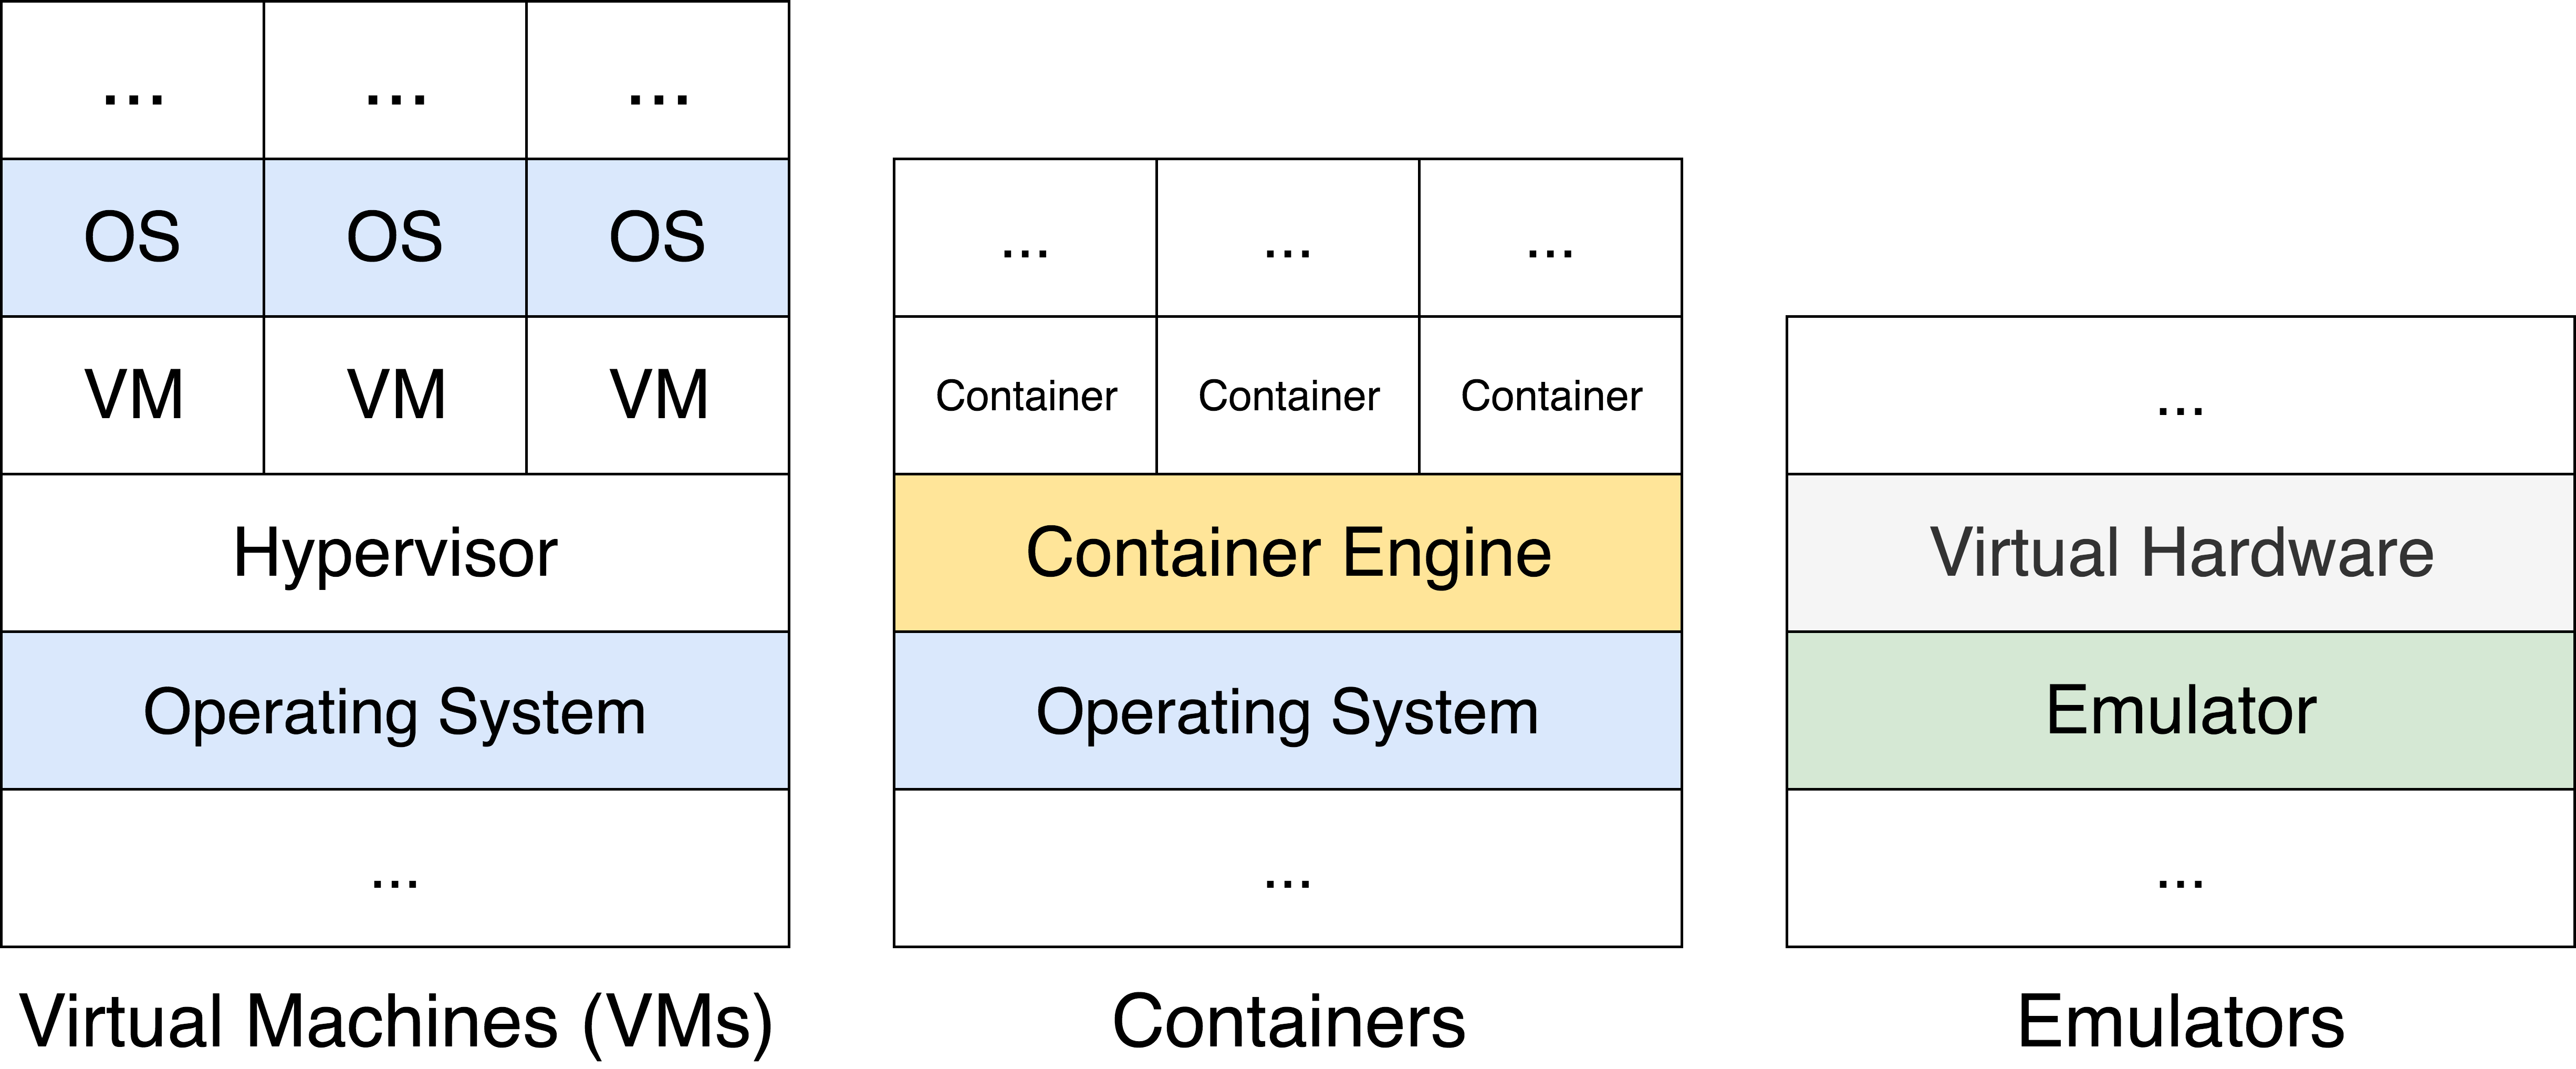
\includegraphics[width=0.70\textwidth]{../figures/vms_containers_emulators.png}
    \caption{Full virtualization is a very resource-hungry process. Containerization is cheaper, as it shares a kernel with the host OS. Emulation lets us emulate hardware as software. Any of these methods can be used in conjunction with any other.\vspace{-10pt}}
    \label{fig:vms_containers_emulators}
\end{figure}

\section{Containerization}\label{sec:containerization}

One of the challenges of distributed software development across heterogeneous platforms is the problem of variability. With today's increasing pace of software development comes the added burden of software maintenance. As hardware and software stacks evolve, source code must periodically be updated to build and run correctly. Maintaining a stable and well-documented codebase can be a considerable challenge, especially in an academic setting where contributors are frequently joining and leaving a project. Together, these challenges present significant obstacles to experimental reproducibility and scientific collaboration.

\begin{figure}[ht]
    \centering
    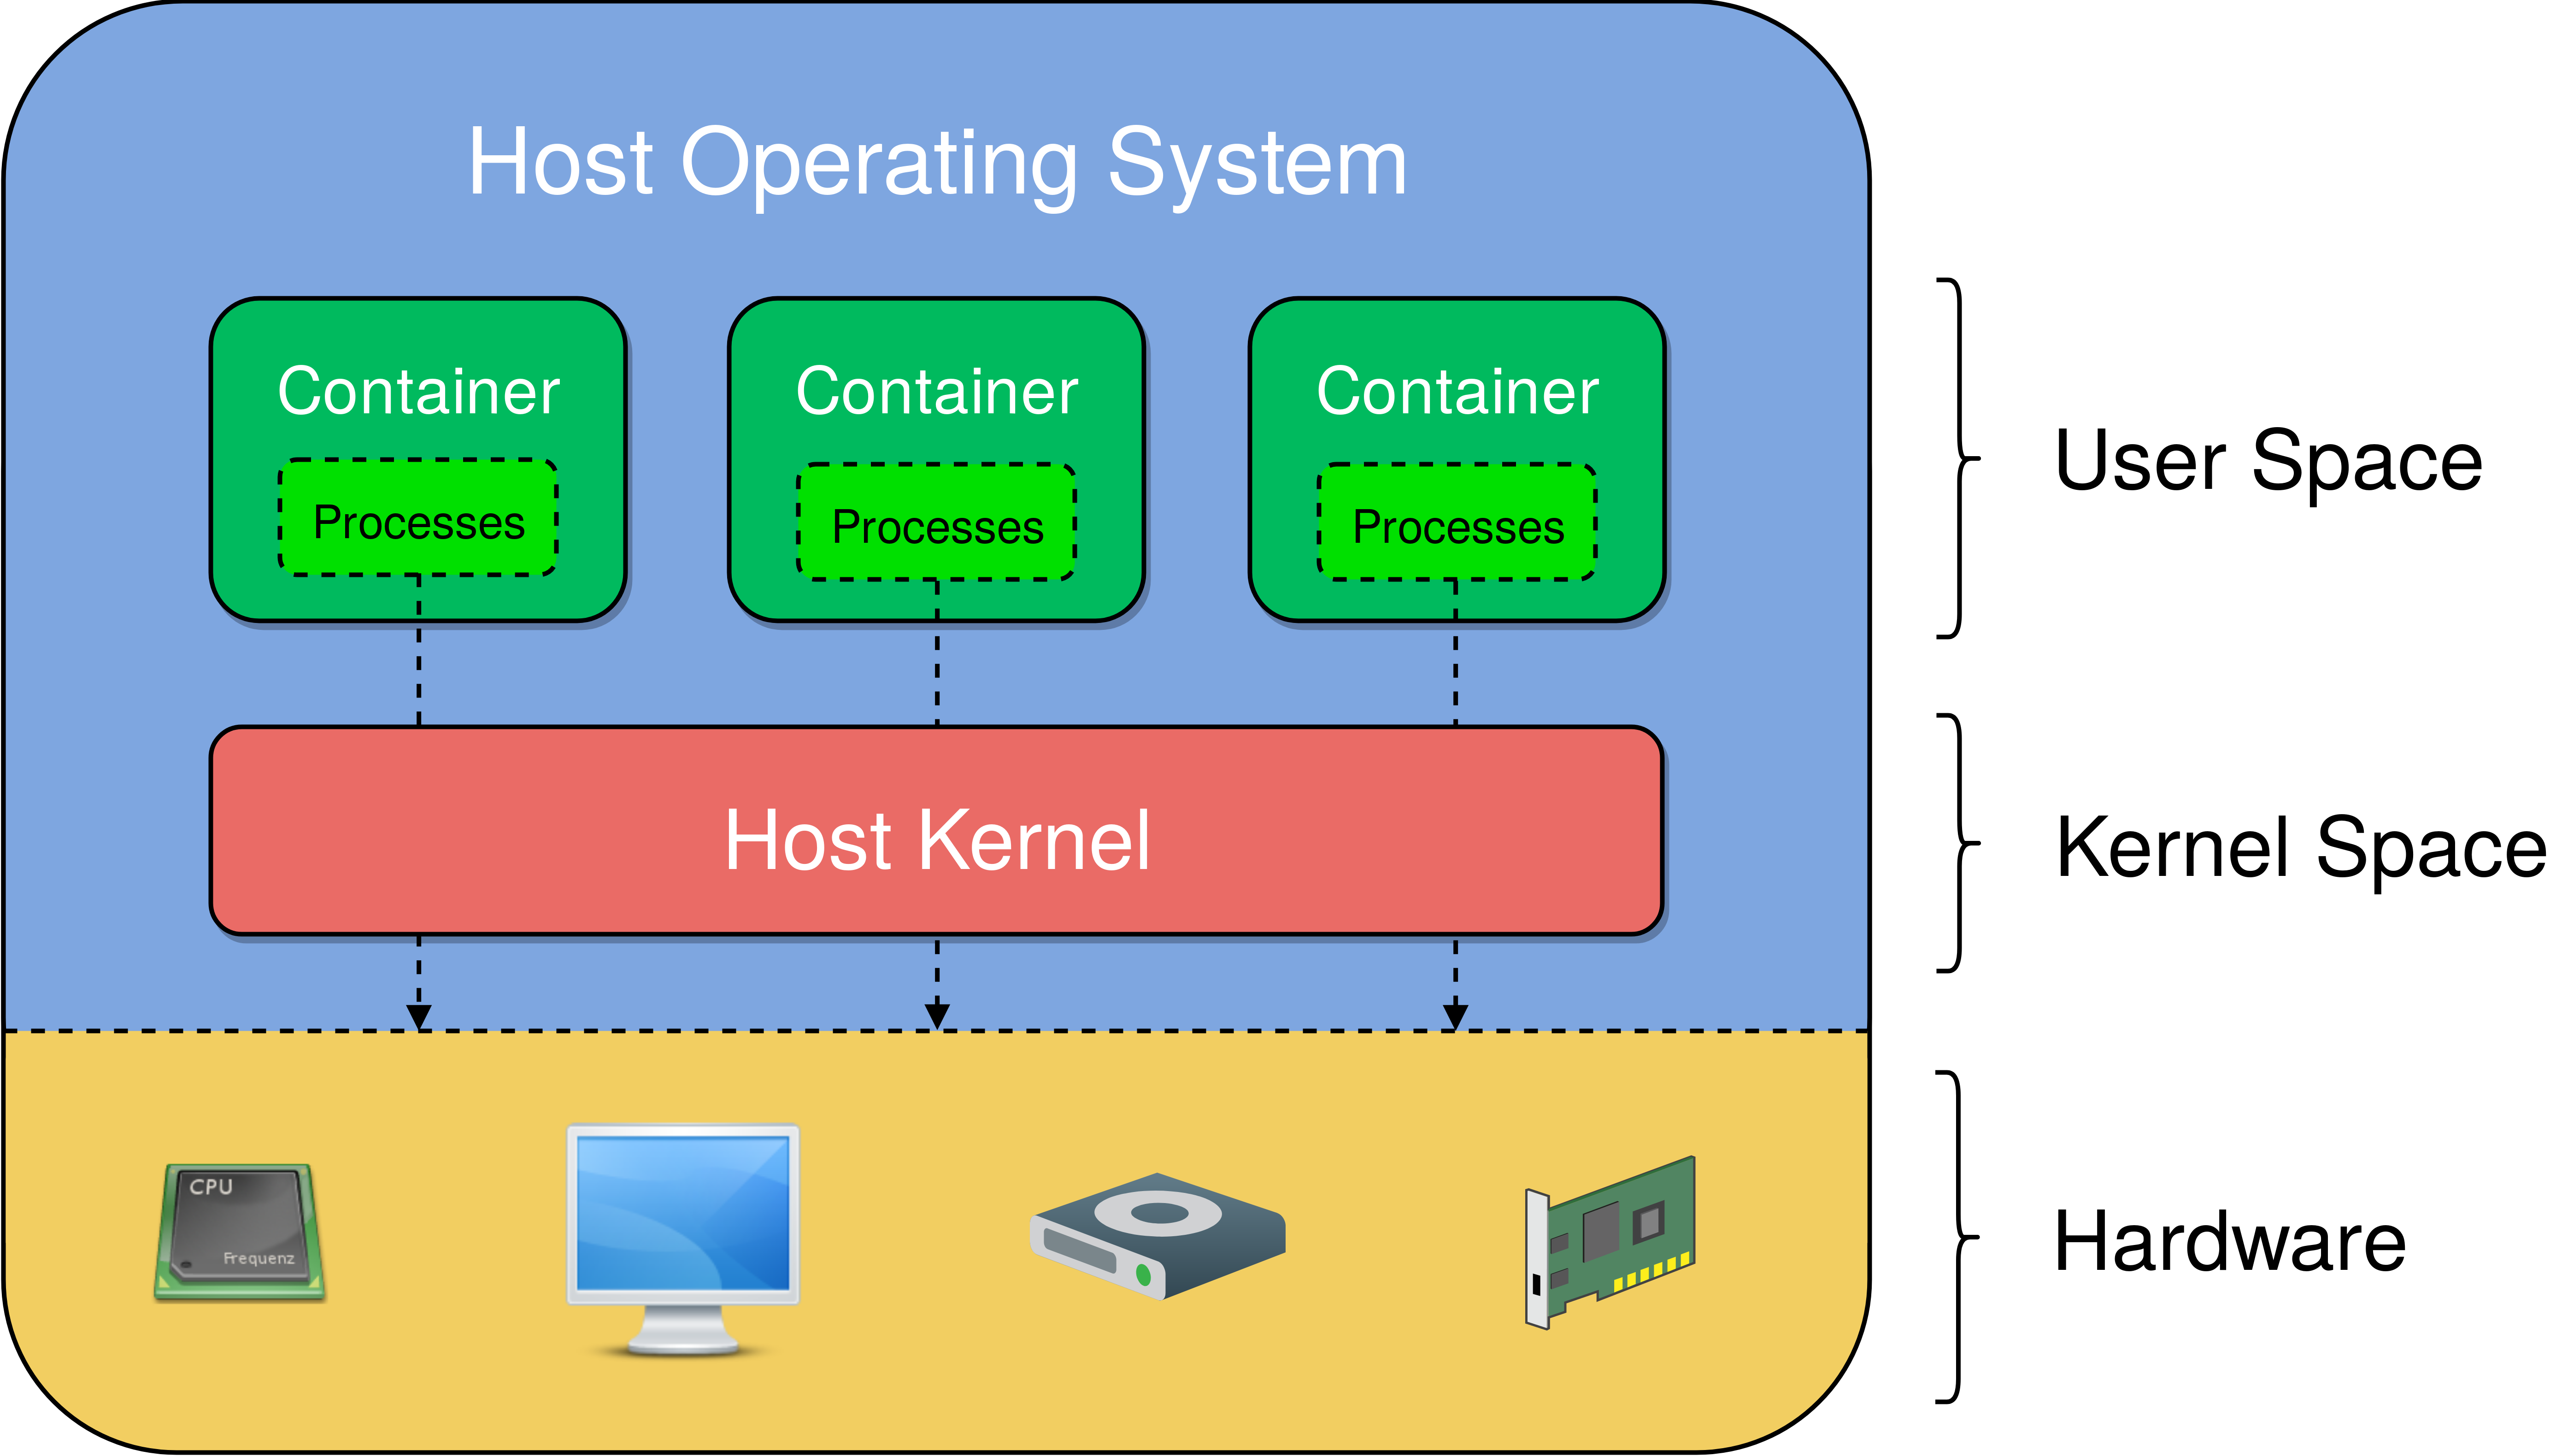
\includegraphics[width=0.65\textwidth]{../figures/user_kernel_hardware.png}
    \caption{Containers live in user space. By default they are sandboxed from the host OS and sibling containers, but unlike VMs, share a common kernel with each other and the host OS. All system calls are passed through host kernel.}
    \label{fig:user_kernel_hardware}
\end{figure}

Docker containers are sandboxed runtime environments that are portable, reproducible and version-controlled. Each environment fully contains its dependencies, but remains isolated from the host OS and file system. Docker provides a mechanism to control the resources each container is permitted to access, and provisions a separate Linux namespace for each container, effectively isolating the network, users, and file system mounts from the host OS. Unlike virtual machines, container-based virtualization tools like Docker are suitable for portable SBCs and can run with close to zero overhead compared to native Linux processes. A single Raspberry Pi is capable of simultaneously running hundreds of containers with no noticeable degradation in performance.\hspace{-.08em}\footnote{\url{https://blog.docker.com/2015/09/update-raspberry-pi-dockercon-challenge/}}

While containerization considerably simplifies the process of building and deploying applications, it also introduces some additional complexity in the software development lifecycle. Docker, like most container platforms, uses a layered filesystem. This enables Docker to take an existing ``image'' and change it by installing new dependencies or modifying its functionality. Images are typically constructed as a sequence of layers, each of which must periodically be updated. Care is required when designing the development pipeline to ensure that such updates do not silently break a subsequent layer, as we describe in \autoref{sec:retrospective}.

\section{Introduction to Docker}\label{sec:docker-intro}

Suppose there is a program which is known to run on some computer. It would be nice to give another computer -- any computer with an internet connection -- a short string of ASCII characters, press \keys{\return}, and return to see that same program running. Never mind where the program was built or what software happened to be running at the time. This may seem trivial, but is a monumental software engineering problem. Various package managers have attempted to solve this, but even when they work as intended, only support natively compiled binaries on operating systems with the same package manager.

Docker\footnote{The following tutorial uses Docker, but the workflow described is similar to most container platforms.} is a tool for portable, reproducible computing. With Docker, users can run any Linux program on almost any networked computing device on the planet, regardless of the underlying operating system or hardware architecture. All of the environment preparation, installation and configuration steps can be automated from start to finish. Depending on how much network bandwidth is available, it might take some time, but users will never need to intervene in the installation process.

To install Docker itself, execute the following command on a POSIX-compliant shell of any \href{https://docs.docker.com/install/#supported-platforms}{Docker-supported platform}:

\begin{pclisting}
    ~$ curl -sSL https://get.docker.com/ | sh
\end{pclisting}
%
A Docker \textit{image} is basically a filesystem snapshot -- a single file that contains everything needed to run a certain Docker container. Docker images are hosted in \textit{registries}, similar to Git repositories or VCS servers. The following command will fetch a Docker image, e.g. \inline{daphne/duck} from the default \hyperref[subsec:docker_hub]{Docker Hub} repository:

\begin{pclisting}
    ~$ docker pull daphne/duck
\end{pclisting}
%
Every Docker image has an image ID, a name and a tag:

\begin{pclisting}
~$ docker images
REPOSITORY      TAG        IMAGE ID         CREATED       SIZE
daphne/duck     latest     ea2f90g8de9e     1 day ago     869MB
\end{pclisting}
%
To run a Docker container\footnote{When a Docker image is running, it is referred to as a \textit{container}.}, use the following command:

\begin{pclisting}
~$ docker run daphne/duck
\end{pclisting}
%
The following command will verify the container is indeed running:

\begin{pclisting}
~$ docker ps
CONTAINER ID     IMAGE           ...     NAMES
52994ef22481     daphne/duck     ...     happy_hamster
\end{pclisting}
%
Note how Daphne's duck container has an alphanumeric container ID, a base image, and a memorable name, \inline{happy\_hamster}. This name is an alias for the container ID, which can be used interchangeably to refer to the container.

Docker images can be created two different ways. First, in \autoref{subsec:creating-an-image-snapshot}, we will see how to create a Docker image by taking a snapshot from a running container, then in \autoref{subsec:writing-an-image-recipe}, how to create a new Docker container using a special kind of recipe, called a \href{https://docs.docker.com/engine/reference/builder/}{\inline{Dockerfile}}.

\subsection{Creating an image snapshot}\label{subsec:creating-an-image-snapshot}

When a Docker container writes to its own filesystem, those changes are not persisted unless committed to a new image. For example, start a container with an interactive shell:

\begin{pclisting}
~$ docker run -it daphne/duck /bin/bash
root@295fd7879184:/#
\end{pclisting}
%
Note the container ID: \inline{295fd7879184}. If we write to disk and leave the container,

\begin{pclisting}
root@295fd7879184:/# touch new_file && ls -l
total 0
-rw-r--r-- 1 root root 0 May 21 20:52 new_file
root@295fd7879184:/# exit
\end{pclisting}
%
\inline{new\_file} will not be persisted. If we re-run the same command again:

\begin{pclisting}
~$ docker run -it daphne/duck /bin/bash
root@18f13bb4571a:/# ls
root@18f13bb4571a:/# touch new_file1 && ls -l
total 0
-rw-r--r-- 1 root root 0 May 21 21:32 new_file1
\end{pclisting}
%
It seems like \inline{new\_file} has disappeared! Notice how the container ID (\inline{18f13bb4571a}) is now different. This is because the command \inline{docker run daphne/duck} created a new container from the base image \inline{daphne/duck}, rather than restarting the previous container. To see all containers on a Docker host, run the following command:

\begin{pclisting}
~$ docker container ls -a
CONTAINER ID      IMAGE            STATUS             NAMES
295fd7879184      daphne/duck      Exited (130)       merry_manatee
18f13bb4571a      daphne/duck      Up 5 minutes       shady_giraffe
52994ef22481      daphne/duck      Up 10 minutes      happy_hamster
\end{pclisting}
%
It appears \inline{295fd7879184} a.k.a. \inline{merry\_manatee} survived, but it is no longer running. Whenever a container's main process (recall we ran \inline{merry\_manatee} with \inline{/bin/bash}) finishes, the container will stop, but it will not cease to exist. In fact, we can resume the stopped container right where it left off:
%
\begin{pclisting}
~$ docker start -a merry_manatee
root@295fd7879184:/# ls -l
total 0
-rw-r--r-- 1 root root 0 May 21 20:52 new_file
\end{pclisting}
%
Nothing was lost! To verify this, we can check which other containers are running:

\begin{pclisting}
~$ docker ps
CONTAINER ID       IMAGE             ...       NAMES
295fd7879184       daphne/duck       ...       merry_manatee
18f13bb4571a       daphne/duck       ...       shady_giraffe
52994ef22481       daphne/duck       ...       happy_hamster
\end{pclisting}
%
Now suppose we would like to share the container \inline{shady\_giraffe} with someone else. To do so, we must first snapshot the running container, or commit it to a new image with a name and a tag. This will create a checkpoint that we may later restore:

\begin{pclisting}
~$ docker commit -m "forking daphne/duck" shady_giraffe user/duck:v2
\end{pclisting}
%
To refer to the container, we can either use \inline{18f13bb4571a} or the designated name (i.e. \inline{shady\_giraffe}). This image repository will be called \inline{user/duck}, and has an optional version identifier, \inline{:v2}, which can be pushed to the \hyperref[subsec:docker_hub]{Docker Hub} registry:

\begin{pclisting}
~$ docker push user/duck:v2
~$ docker images
REPOSITORY    TAG        IMAGE ID         CREATED          SIZE
daphne/duck   latest     ea2f90g8de9e     1 day ago        869MB
user/duck     v2         d78be5cf073e     2 seconds ago    869MB
~$ docker pull user/duck:v2
~$ docker run user/duck ls -l
total 0
-rw-r--r-- 1 root root 0 May 21 21:32 new_file1
\end{pclisting}
%
This is a convenient way to share an image with colleagues and collaborators. Anyone with access to the repository can pull this image and continue where we left off, or create another image based on top.

\subsection{Writing an image recipe}\label{subsec:writing-an-image-recipe}

The second way to create a Docker image is to write a recipe, called a \inline{Dockerfile}. A \inline{Dockerfile} is a text file that specifies the commands required to create a Docker image, typically by modifying an existing container image using a scripting interface. They also have special \href{https://docs.docker.com/engine/reference/builder/}{keywords} (which are conventionally \inline{CAPITALIZED}), like \href{https://docs.docker.com/engine/reference/builder/#from}{\inline{FROM}}, \href{https://docs.docker.com/engine/reference/builder/#from}{\inline{RUN}}, \href{https://docs.docker.com/engine/reference/builder/#entrypoint}{\inline{ENTRYPOINT}} and so on. For example, create a file called \inline{Dockerfile} with the following content:

\begin{dockerlisting}
FROM daphne/duck      # Defines the base image
RUN touch new_file1   # new_file1 will be part of our snapshot
CMD ls -l             # Default command run when container is started
\end{dockerlisting}
%
Now, to build the image, we can simply run:

\begin{pclisting}
~$ docker build -t user/duck:v3 (*@\hl{.}@*)
\end{pclisting}
%
The \inline{.} indicates the current directory, which should be the same one containing our \inline{Dockerfile}. This command should produce something like the following output:

\begin{pclisting}
Sending build context to Docker daemon  2.048kB
Step 1/3 : FROM daphne/duck
--- ea2f90g8de9e
Step 2/3 : RUN touch new_file1
--- e3b75gt9zyc4
Step 3/3 : CMD ls -l
--- Running in 14f834yud59
Removing intermediate container 14f834yud59
--- 05a3bd381fc2
Successfully built 05a3bd381fc2
Successfully tagged user/duck:v3
\end{pclisting}
%
The command, \inline{docker images} should display an image called \inline{user/duck:v3}:

\begin{pclisting}
~$ docker images
REPOSITORY    TAG        IMAGE ID         CREATED          SIZE
daphne/duck   latest     ea2f90g8de9e     1 day ago        869MB
user/duck     v2         d78be5cf073e     5 minutes ago    869MB
user/duck     v3         05a3bd381fc2     2 seconds ago    869MB
\end{pclisting}
%
This procedure is identical to the snapshot technique performed in \autoref{subsec:creating-an-image-snapshot}, but the result is cleaner. Rather than maintaining a 869 MB image, we can just store the 4 KB text file instead. To run the resulting image, we can simply use the same command as before:

\begin{pclisting}
~$ docker run -it user/duck:v3
total 0
-rw-r--r-- 1 root root 0 May 21 21:35 new_file1
\end{pclisting}
%
Notice that as soon as we run the container, Docker will execute the \inline{ls -l} command as specified by the \inline{Dockerfile}, revealing that \inline{new\_file1} was indeed stored in the image. However, this default command can be overridden by supplying a custom command:

\begin{pclisting}
~$ docker run -it user/duck:v3 [custom_command]
\end{pclisting}
%
\subsection{Layer Caching}

\href{https://docs.docker.com/storage/storagedriver/#images-and-layers}{Layers} are an important concept to understand when working with Docker. One way to think of a layer is like a Git commit -- a set of changes to a previous image or layer, uniquely identified by a hash code. In a \inline{Dockerfile}, layers begin with a \href{https://docs.docker.com/engine/reference/builder/#from}{keyword}.

\begin{dockerlisting}
FROM daphne/duck
RUN touch new_file1                            # Defines a new layer
RUN mkdir config && mv new_file1 config        # Layers can chain commands
RUN apt-get update && apt-get install -y wget  # Install a dependency
RUN wget https://get.your.app/install.sh       # Download a script
RUN chmod +x install.sh && ./install.sh        # Run the script
\end{dockerlisting}
%
To build this image, we can run the following command:

\begin{pclisting}
~$ docker build -t user/duck:v4 .
Sending build context to Docker daemon  2.048kB
Step 1/6 : FROM daphne/duck
---> cd6d8154f1e1
...
Removing intermediate container 8fb56ef38bc8
---> 3358ca1b8649
Step 5/6 : RUN wget https://get.your.app/install.sh
---> Running in e8284ff4ec8b
...
2018-10-30 06:47:57 (89.9 MB/s) - 'install.sh' saved [13847/13847]
Removing intermediate container e8284ff4ec8b
---> 24a22dc2900a
Step 6/6 : RUN chmod +x install.sh && ./install.sh
---> Running in 9526651fa492
# Executing install script, commit: 36b78b2
...
Removing intermediate container 9526651fa492
---> a8be23fea573
Successfully built a8be23fea573
Successfully tagged user/duck:v4
\end{pclisting}
%
Layers are conveniently cached by the \href{https://docs.docker.com/engine/reference/commandline/dockerd/}{Docker daemon}. Should we need to run the same command twice, Docker will use the cache instead of rebuilding the entire image:

\begin{pclisting}
Sending build context to Docker daemon  2.048kB
Step 1/6 : FROM daphne/duck
---> cd6d8154f1e1
Step 2/6 : RUN touch new_file1
---> Using cache
---> 0473154b2004
...
Step 6/6 : RUN chmod +x index.html && ./index.html
---> Using cache
---> a8be23fea573
Successfully built a8be23fea573
Successfully tagged user/duck:v4
\end{pclisting}
%
If we need to make a change to the \inline{Dockerfile}, Docker will only rebuild the image starting from the first modified step. Suppose we were to add a new \inline{RUN} command at the end of our \inline{Dockerfile} and trigger a rebuild like so:

\begin{pclisting}
~$ echo 'RUN echo "Change here!"' >> Dockerfile
~$ docker build -t user/duck:v4 .
Sending build context to Docker daemon  2.048kB
...
Step 6/7 : RUN chmod +x index.html && ./index.html
---> Using cache
---> a8be23fea573
Step 7/7 : RUN echo "Change here!"
---> Running in 80fc5c402304
Change here!
Removing intermediate container 80fc5c402304
---> c1ec64cef9c6
Successfully built c1ec64cef9c6
Successfully tagged user/duck:v4
\end{pclisting}
%
If Docker had to rerun the entire \inline{Dockerfile} from top to bottom each time it was rebuilt, this would be slow and inconvenient. Instead, Docker caches the unmodified steps by default, and only reruns the minimum set of steps necessary to rebuild. This can sometimes introduce unexpected results, especially when the cache is stale. To ignore the cache and force a clean rebuild, use the \inline{-{}-no-cache} flag when building a \inline{Dockerfile}.

What does Docker consider when deciding whether to use the cache? First is the \inline{Dockerfile} itself -- when a step in a \inline{Dockerfile} changes, both it and any subsequent steps will need to be rerun during a build. Docker also checks the \href{https://docs.docker.com/engine/reference/commandline/build/#extended-description}{build context} for changes. When \inline{docker build -t TAG .} is written, the \inline{.} indicates the build context, or path where the build should occur. Often, this path contains build artifacts. For example:

\begin{dockerlisting}
FROM daphne/duck
COPY duck.txt .
RUN cat duck.txt
\end{dockerlisting}
%
Now if we add some message in \inline{duck.txt} and rebuild our image, the file will be copied into the Docker image, and its contents will be printed:

\begin{pclisting}
~$ echo "Make way!" > duck.txt && docker build -t user/duck:v5 .
Sending build context to Docker daemon  3.072kB
Step 1/3 : FROM daphne/duck
---> cd6d8154f1e1
Step 2/3 : COPY duck.txt .
---> e0e03d9e1791
Step 3/3 : RUN cat duck.txt
---> Running in 590c5420ce29
Make way!
Removing intermediate container 590c5420ce29
---> 1633e3e10bef
Successfully built 1633e3e10bef
Successfully tagged user/duck:v5
\end{pclisting}
%
As long as the first three lines of the \inline{Dockerfile} and \inline{duck.txt} are unmodified, these layers will be cached and Docker will not rebuild them. If the contents of the file \inline{duck.txt} are subsequently modified, this will trigger a rebuild to occur. For example, if we append to the file and rebuild, only the last two steps will need to be executed:

\begin{pclisting}
~$ echo "Thank you. Have a nice day!" >> duck.txt
~$ docker build -t user/duck:v5 .
Sending build context to Docker daemon  3.072kB
Step 1/3 : FROM ubuntu
---> cd6d8154f1e1
Step 2/3 : COPY duck.txt .
---> f219efc150a5
Step 3/3 : RUN cat duck.txt
---> Running in 7c6f5f8b73e9
Make way!
Thank you. Have a nice day!
Removing intermediate container 7c6f5f8b73e9
---> e8a1db712aee
Successfully built e8a1db712aee
Successfully tagged user/duck:v5
\end{pclisting}
%
A common mistake when writing \inline{Dockerfile}s is to \inline{COPY} more files than are strictly necessary to perform the following build step. For example, if \inline{COPY . .} is written at the beginning of the \inline{Dockerfile}, whenever any file is changed within the build context, this will trigger a rebuild of all subsequent build steps. In order to maximize cache reusability and minimize rebuild time, users should be as conservative as possible and only \inline{COPY} the minimum set of files necessary to accomplish the following build step.

% Like Git's \inline{.gitignore}, Docker also has a \inline{.dockerignore} file. If we add a line to the \inline{.dockerignore} file, then all paths matching this line in the build context will be ignored. Docker also accepts other patterns like regular expressions and negation.~\footnote{Further details: \url{https://docs.docker.com/engine/reference/builder/#dockerignore-file}}

\subsection{Volume Sharing}\label{subsec:volume_sharing}

There is a second method of depositing data into a container, which does not require baking it into the parent image at compile-time. This method is more appropriate for data which is required at runtime, but non-essential for the build. It takes the following form:

\begin{pclisting}
~$ docker run user/duck:v6 (*@\hl{-v HOST\_PATH:TARGET\_PATH}@*)
\end{pclisting}
%
Suppose we have a \inline{Dockerfile} which provides a default \inline{CMD} instruction:

\begin{dockerlisting}
FROM daphne/duck
CMD /bin/bash -c "/launch.sh"
\end{dockerlisting}
%
If we built this image and tried to run it, the file \inline{launch.sh} would be missing:

\begin{pclisting}
~$ docker build -t user/duck:v6 && docker run user/duck:v6
bash: /launch.sh: No such file or directory
\end{pclisting}
%
Instead, when running the container, we need to share the file via the Docker CLI:

\begin{pclisting}
~$ echo -e '#!/bin/bash\necho Launching...' >> launch.sh && \
   chmod 775 launch.sh && \
   docker run user/duck:v6 (*@\hl{-v launch.sh:/launch.sh}@*)
Launching...
\end{pclisting}
%
This way, the local file \inline{launch.sh} will be available to use from within the container at the designated path, \inline{/launch.sh}.

\subsection{Multi-stage builds}

Docker's filesystem is additive, so each layer will only increase the size of the final image. For this reason, it is often necessary to tidy up unneeded files after installation. For example, when installing dependencies on Debian-based images, it is a common practice to run:

\begin{dockerlisting}
RUN apt-get update && apt-get install ... && (*@\hl{rm -rf /var/lib/apt/lists/*}@*)
\end{dockerlisting}
%
This ensures the package list is not baked into the image (Docker will only checkpoint the layer after each step is complete). Builds can often consume several steps, despite only producing a single artifact. Instead of chaining together several commands and cleaning up changes in a single step, multi-stage builds let us build a series of images inside a \inline{Dockerfile}, and copy resources from one to another, discarding all intermediate build artifacts:

\begin{dockerlisting}
FROM user/duck:v3 as template1

FROM daphne/duck as template2
COPY --from=template1 new_file1 new_file2
FROM donald/duck as template3
COPY --from=template2 new_file2 new_file3
CMD ls -l
\end{dockerlisting}
%
Now we can build and run this image as follows:

\begin{pclisting}
~$ docker build . -t user/duck:v4
Sending build context to Docker daemon  2.048kB
Step 1/6 : FROM user/duck:v3 as template1
--- e3b75ef8ecc4
Step 2/6 : FROM daphne/duck as template2
--- ea2f90g8de9e
Step 3/6 : COPY --from=template1 new_file1 new_file2
---> 72b96668378e
Step 4/6 : FROM donald/duck:v3 as template3
---> e3b75ef8ecc4
Step 5/6 : COPY --from=template2 new_file2 new_file3
---> cb1b84277228
Step 6/6 : CMD ls
---> Running in cb1b84277228
Removing intermediate container cb1b84277228
---> c7dc5dd63e77
Successfully built c7dc5dd63e77
Successfully tagged user/duck:v4
~$ docker run -it user/duck:v4
total 0
-rw-r--r-- 1 root root 0 Jul  8 15:06 new_file3
\end{pclisting}
%
One application of multi-stage builds is compiling a project dependency from its source code. In addition to all the source code, the compilation process could introduce gigabytes of build artifacts and transitive dependencies, just to build a single binary. Multi-stage builds allow us to build the file, and copy it to a fresh layer, unburdened by intermediate files.

\section{ROS and Docker}\label{sec:ros-docker}

\begin{figure}[ht]
\centering
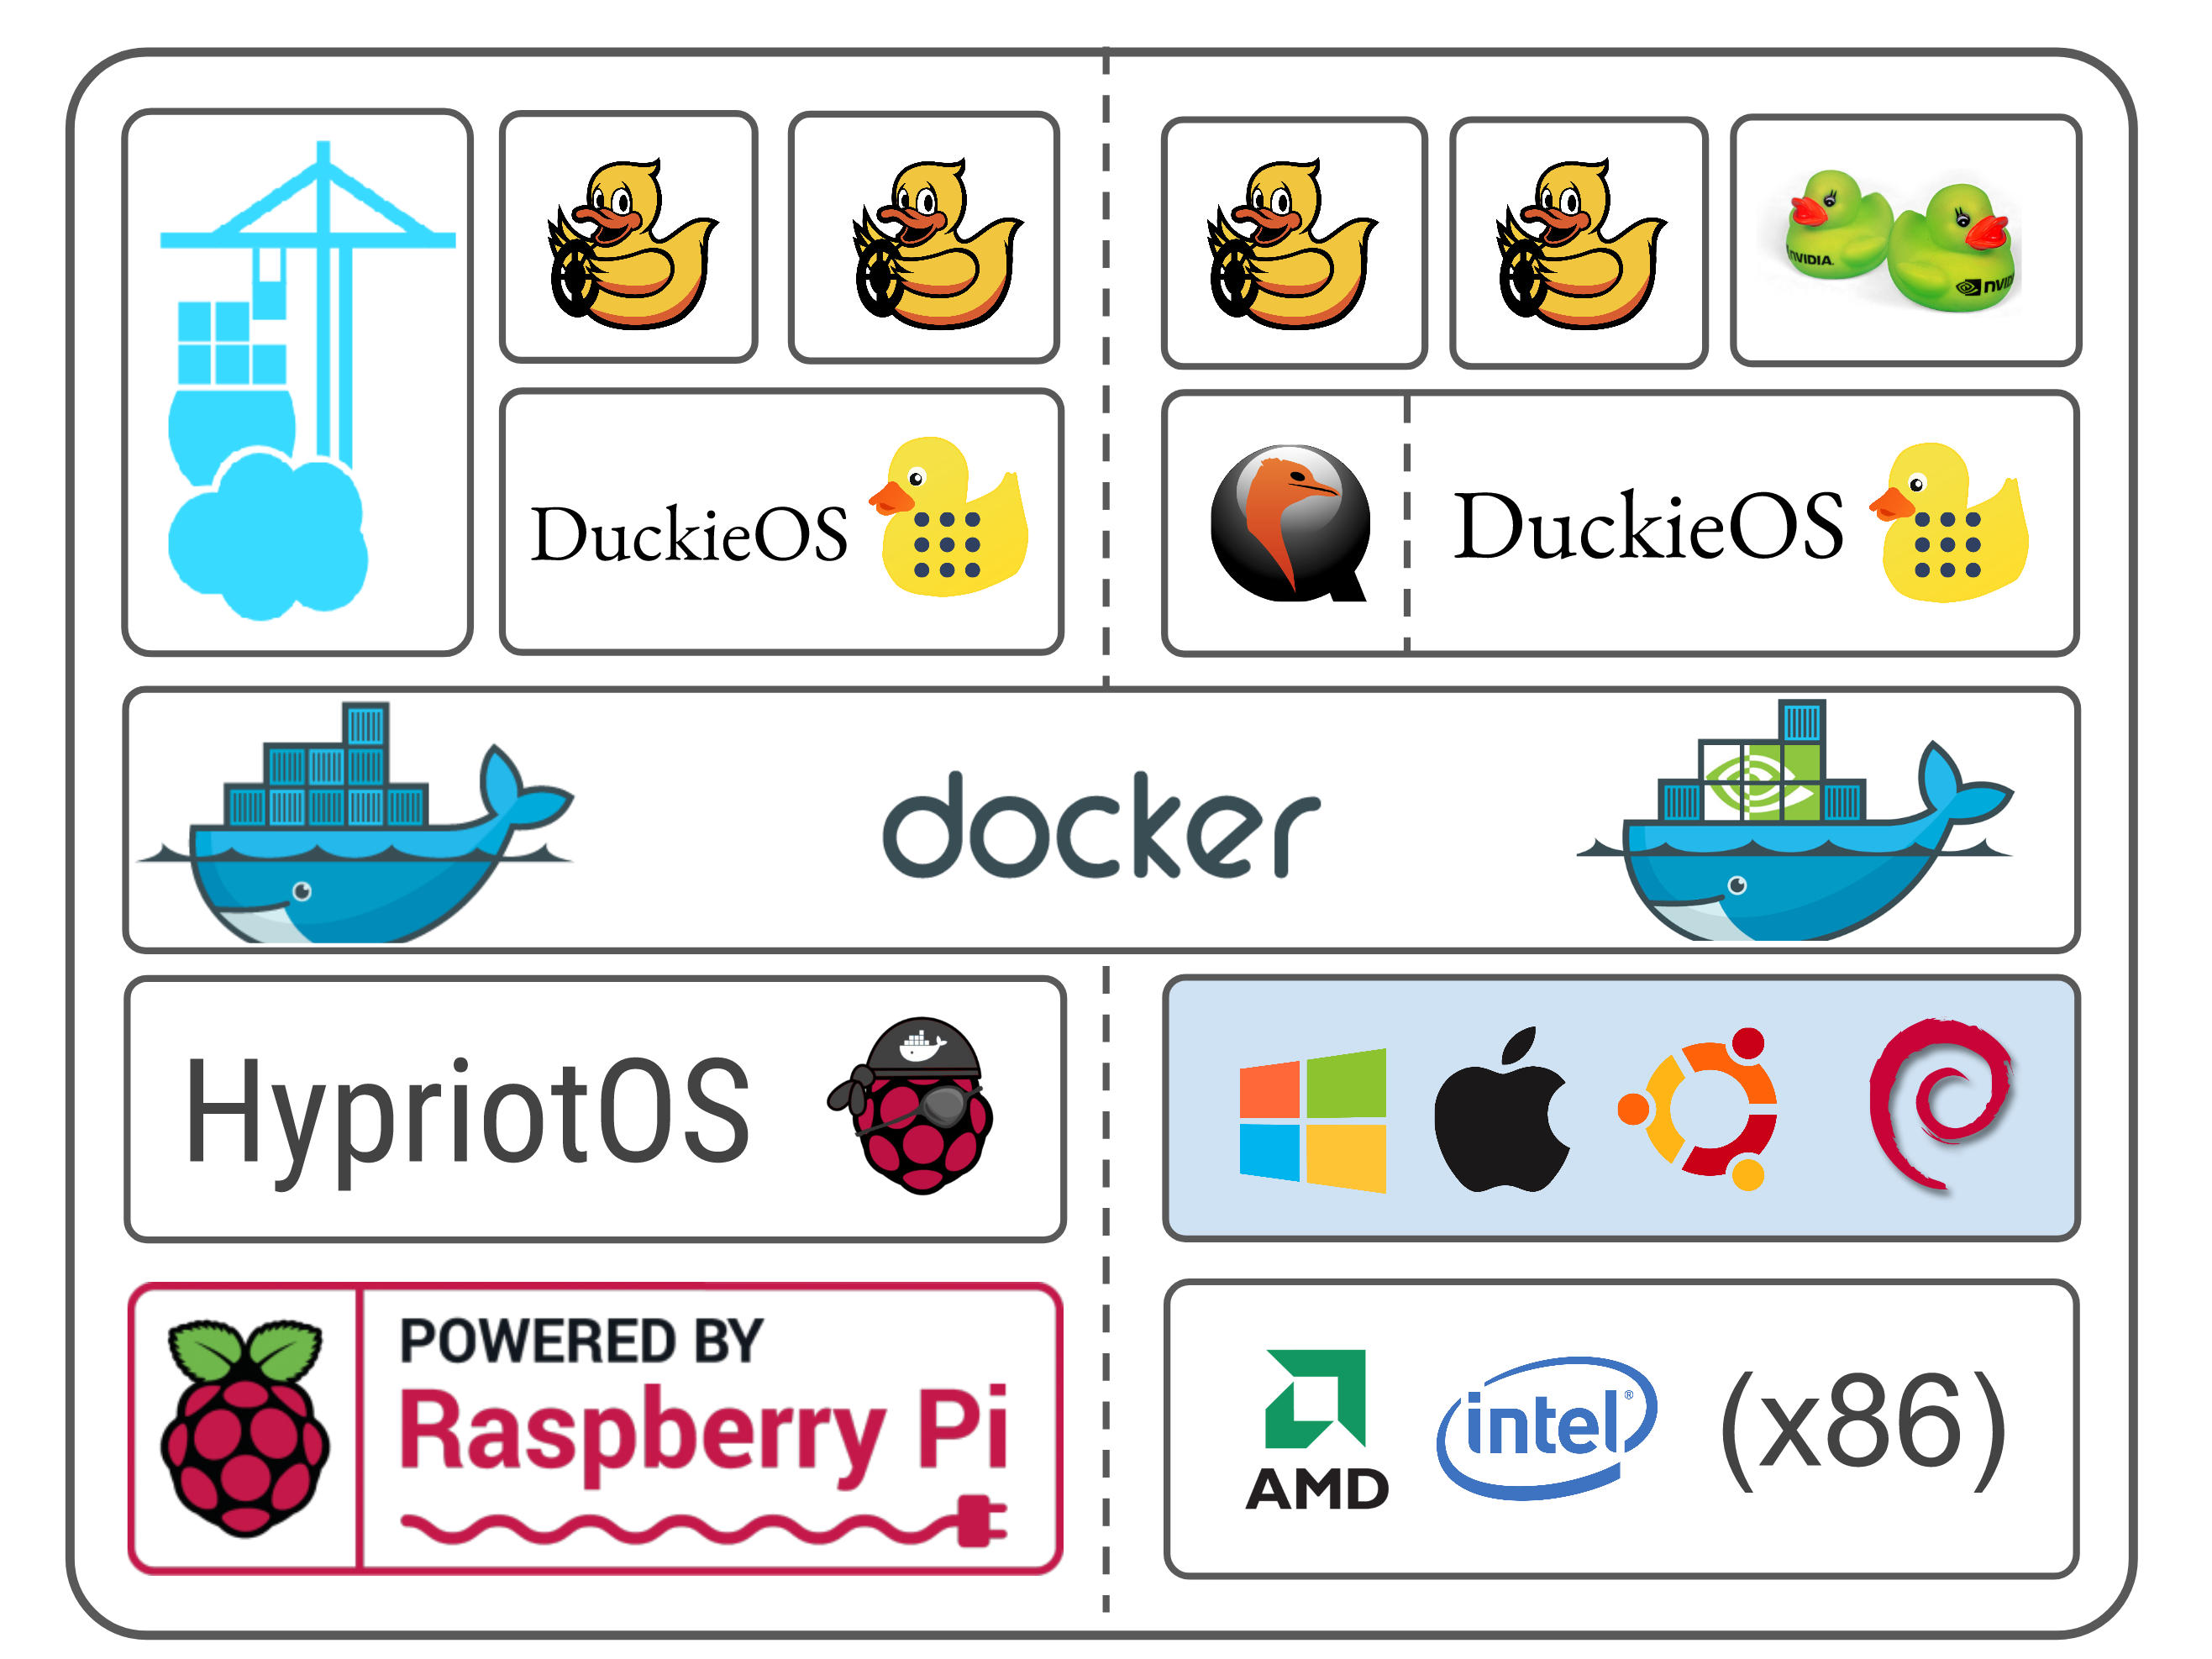
\includegraphics[width=0.48\textwidth]{../figures/docker_stack_1.png}
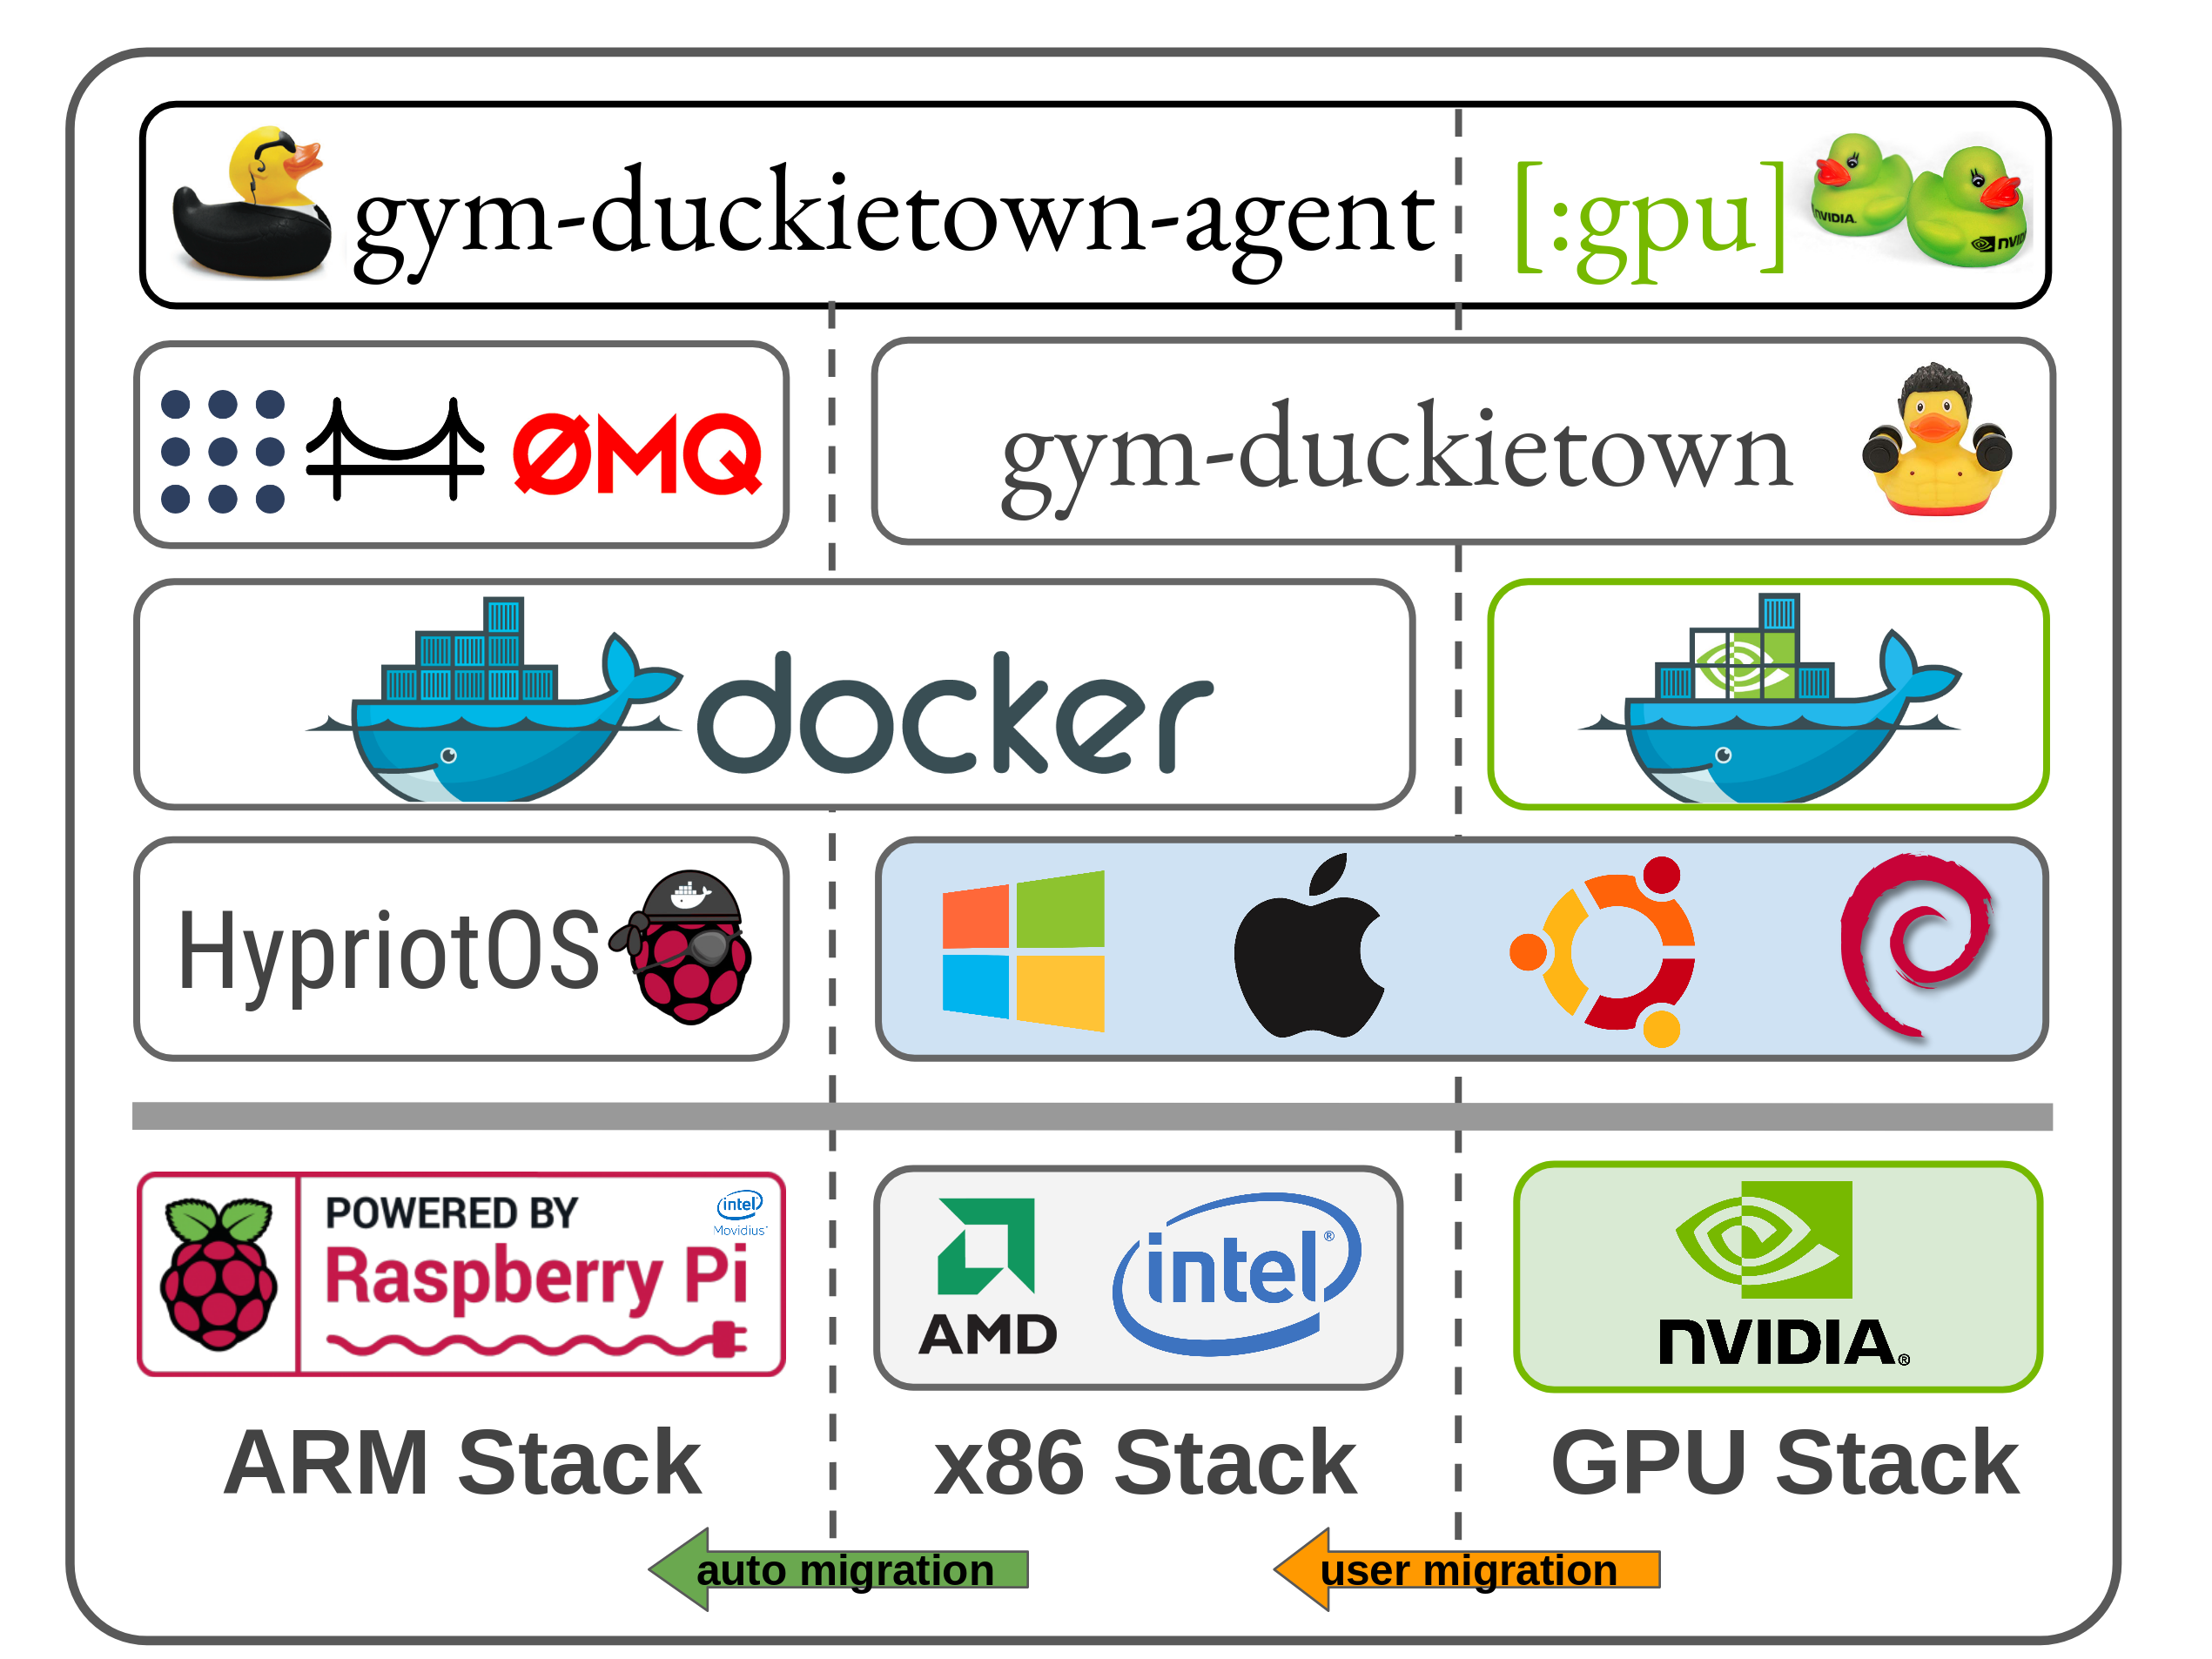
\includegraphics[width=0.48\textwidth]{../figures/docker_stack_2.png}
\caption{Container infrastructure. \textbf{Left}: The ROS stack targets two primary architectures, x86 and ARM. To simplify the build process, we build ARM artifacts on x86 using \href{https://www.qemu.org}{QEMU}~\citep{bellard2005qemu}. \textbf{Right}: Reinforcement learning stack. Build artifacts are trained on a GPU, and transferred to CPU for evaluation. Deep learning models may be also be run on an ARM device using an \href{https://software.intel.com/en-us/neural-compute-stick}{accelerator}.}
\label{fig:docker}
\end{figure}

\citet{white2017ros-docker} previously explored Dockerizing ROS, whose work forms the basis for our own, which extends their implementation to the Duckietown platform~\citep{paull2017duckietown}, a more hardware- and domain-specific set of ROS applications.

The \href{https://www.duckietown.org}{Duckietown platform} supports two primary instruction set architectures: x86 and ARM. To ensure the runtime compatibility of Duckietown packages, we cross-build using hardware virtualization to ensure build artifacts can be run on either target architecture. Runtime emulation of foreign artifacts is also possible, using a similar technique.\hspace{-.08em}\footnote{For more information, this technique is described in further depth at the following URL: \url{https://www.balena.io/blog/building-arm-containers-on-any-x86-machine-even-dockerhub/}.} For performance and simplicity, we only use emulation where necessary (e.g., on x86 devices). On ARM-native, the base operating system is \hyperref[subsec:hypriot]{HypriotOS}, a lightweight Debian distribution for the Raspberry Pi and other ARM-based SBCs, with native support for Docker. For both x86 and ARM-native, Docker is the underlying container platform upon which all user applications are run, inside a container. Since both ROS and Docker have extensive command line interfaces, a unified interface, the \href{https://github.com/duckietown/duckietown-shell}{Duckietown Shell} (\inline{dts}), is provided to wrap their functionality and perform common tasks.

\section{Duckiebot Development using Docker}

\noindent Software development for the Duckietown platform requires the following physical objects:
%
\begin{enumerate}
\item Duckiebot (including custom hat, camera, wheels, and Raspberry Pi 3B+)\footnote{Full materials list can be located at the following URL: \url{https://get.duckietown.org/}}
\item Micro SD card (16GB+ recommended)
\item Personal computer
\item Internet-enabled router
\item MicroSD card adapter
\end{enumerate}
%
In addition, we assume the following software dependencies have been installed on (3):
%
\begin{enumerate}[label=(\alph*)]
\item \href{https://get.docker.com}{Docker CE}
\item POSIX-compliant shell
\item \inline{dts}, the Duckietown shell\footnote{May be obtained at the following URL: \url{https://github.com/duckietown/duckietown-shell}}
\item Web browser (e.g. \href{https://www.google.com/chrome/}{Chrome} or \href{https://mozilla.org/firefox/}{Firefox})
\item \inline{wget}/\inline{curl}
\end{enumerate}

\noindent The following workflow has been tested extensively on Linux hosts running Ubuntu 16.04 (and to a lesser extent, Mac OS X and VMs). No other dependencies are assumed or required.

\subsection{Flashing a bootable disk}

One of the first steps in the Duckiebook requires users to manually install a custom operating system onto bootable media, a tedious and time-consuming process. The following installation script was written to automate this process, allowing users to setup a reproducible software environment more easily:

\begin{pclisting}
~$ bash -c "(*@\$@*)(wget -O- h.ndan.co)"
\end{pclisting}
%
Now, with the \href{https://github.com/duckietown/duckietown-shell}{Duckietown Shell}, the following command is all that is needed:
%
\begin{dtslisting}
dt> init_sd_card [--hostname "DUCKIEBOT_NAME"] [--wifi "username:password"]
\end{dtslisting}
%
Users must insert an SD card and follow the instructions provided. When complete, the card is removed and inserted into the SD card slot on the Raspberry Pi. On first boot, care must be taken to ensure the device is powered continuously for a minimum of ten minutes in order to allow installation to complete and avoid filesystem corruption.

\subsection{Web interface}

To access the DuckieOS web interface, users can visit the following URL in any JavaScript-enabled web browser: \url{http://DUCKIEBOT_NAME:9000/}. If the installation process successfully completed and the network is properly configured, the web application displayed in~\autoref{fig:portainer_ui} should be accessible. This application allows users unfamiliar with the CLI to manage containers on their Duckiebots from within the browser.

\begin{figure}
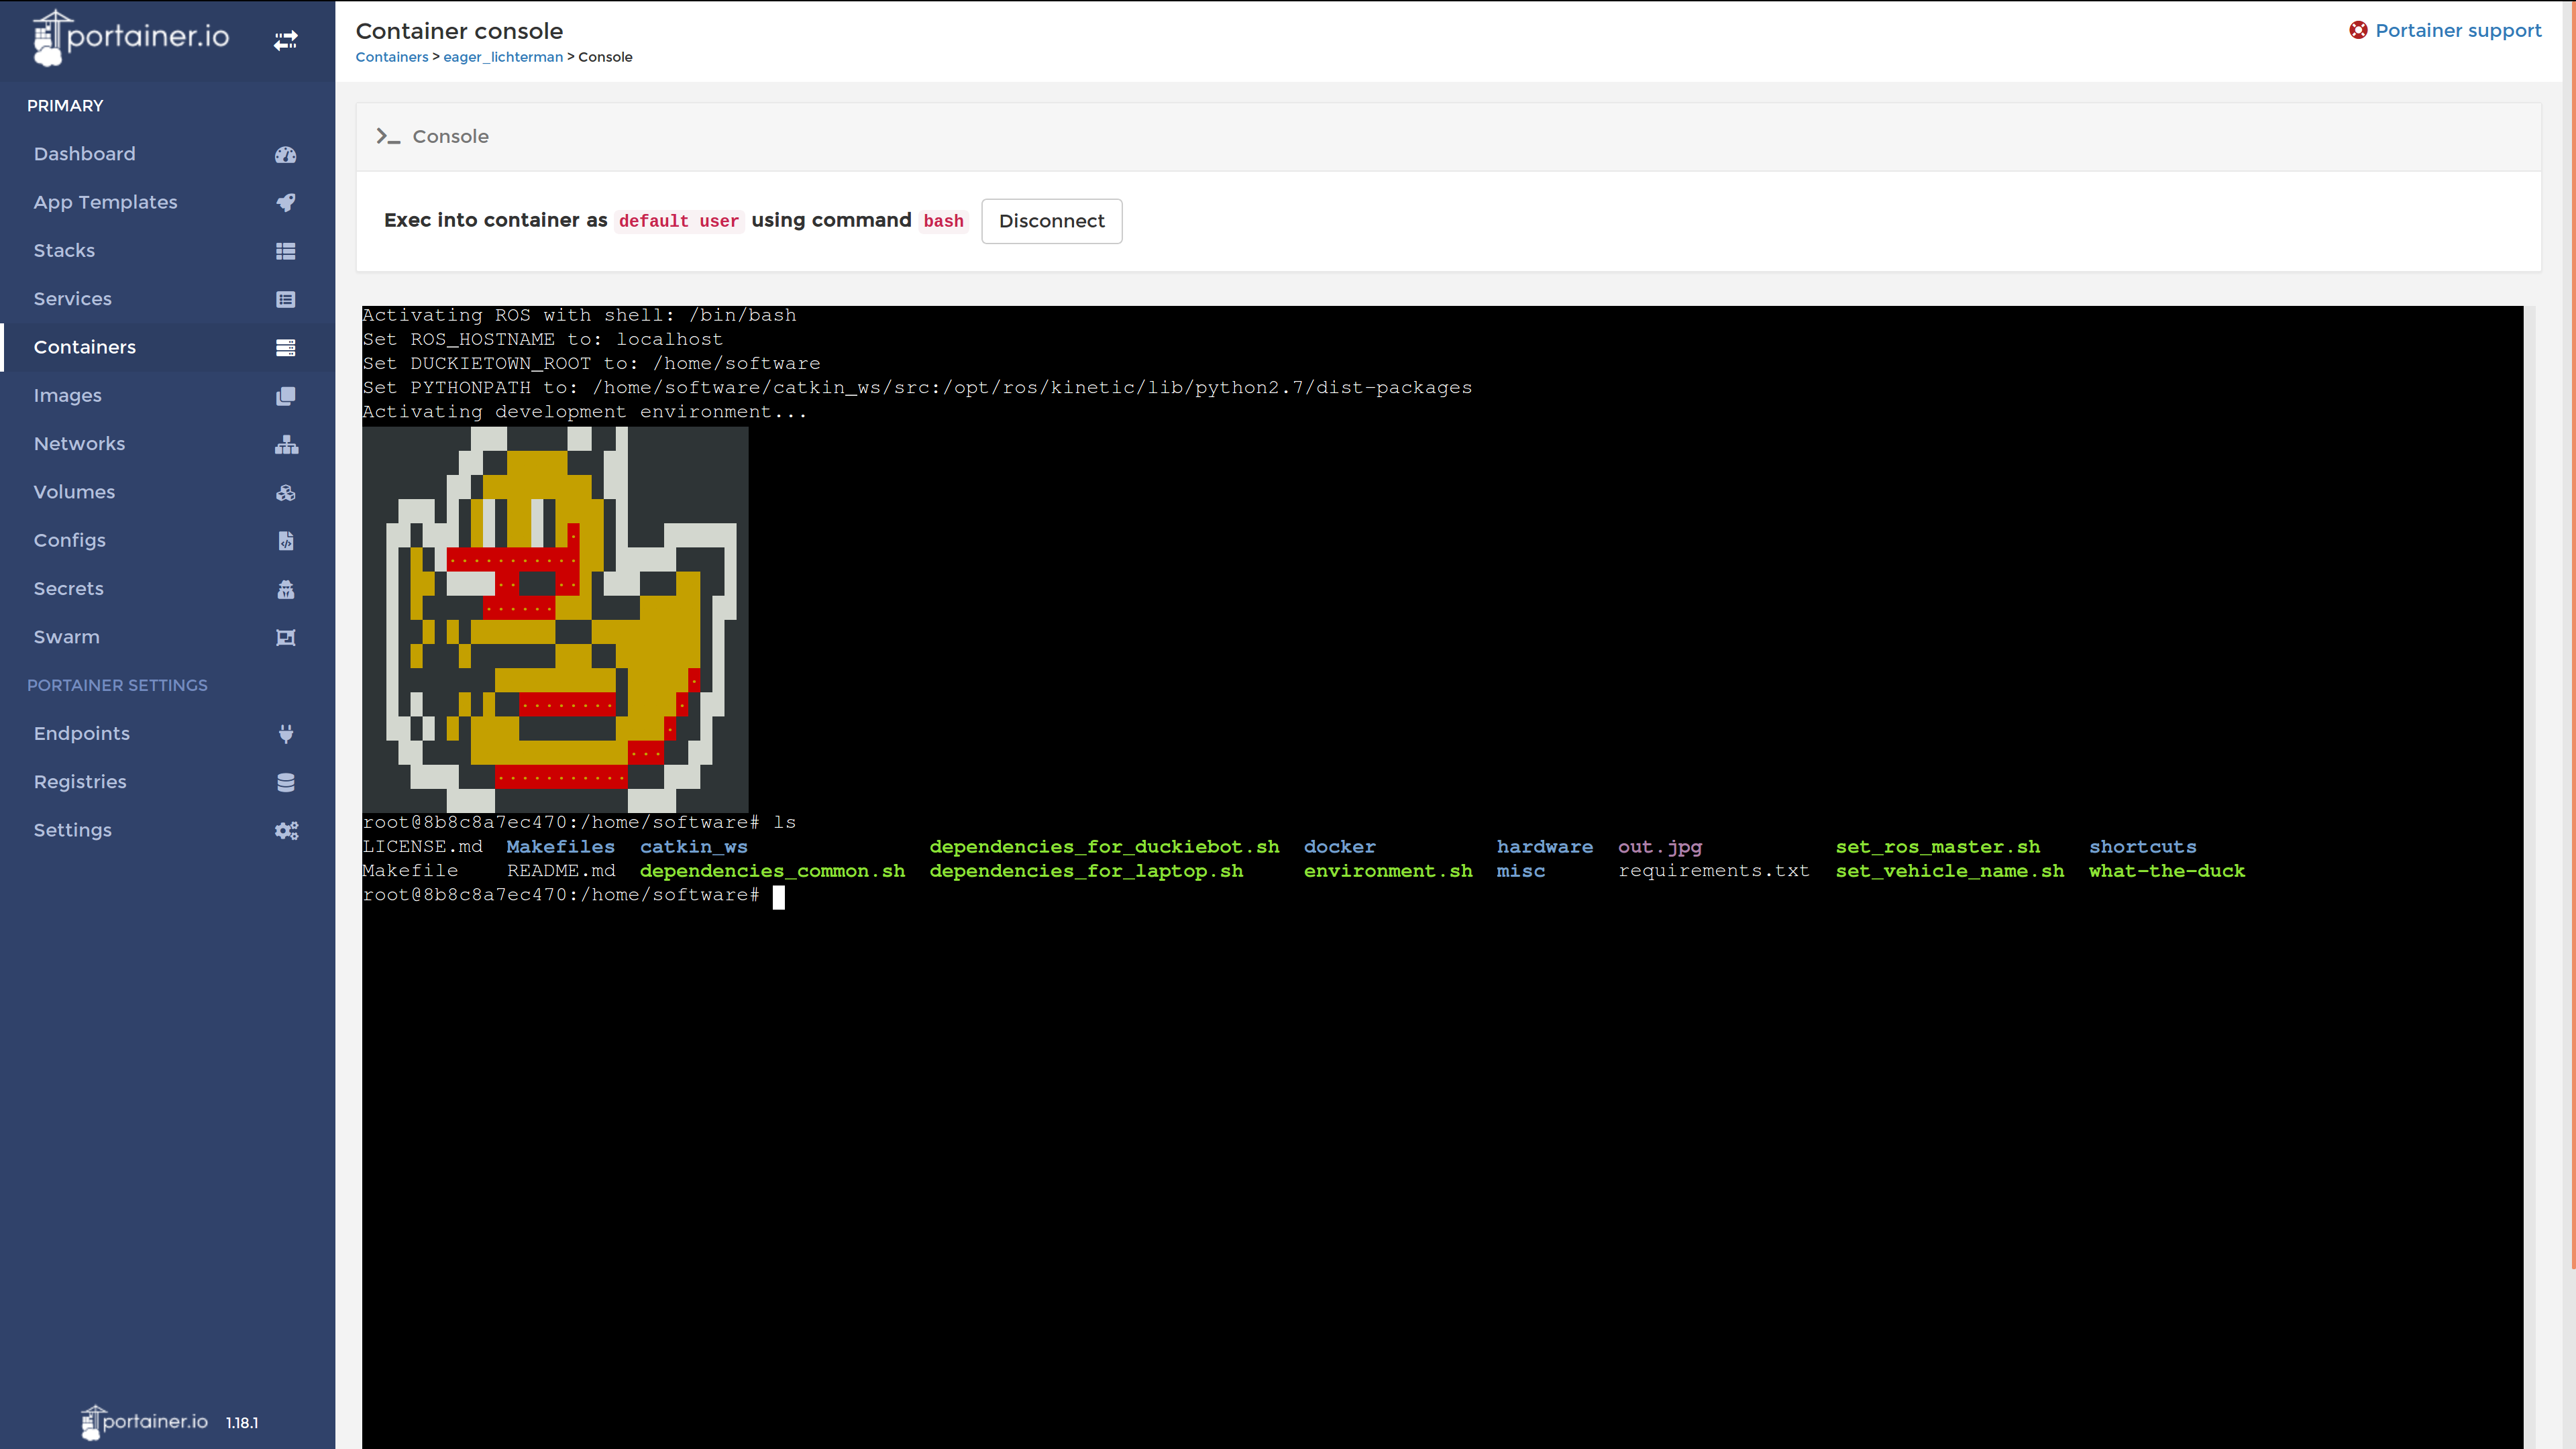
\includegraphics[width=0.80\textwidth]{../figures/portainer_screenshot.png}
\caption{Browser interface for individual Duckiebots. It is provided by \href{https://www.portainer.io/}{Portainer}, a RESTful web dashboard, which wraps the Docker CLI and offers support for container management, configuration, networking and terminal emulation (shown above). \menu{{\url{http://DUCKIEBOT_NAME:9000/#/container/container_name}} > ``\underline{Console}'' \faMousePointer}}
\label{fig:portainer_ui}
\end{figure}

\subsection{Testing ROS}

\noindent To verify Docker is working properly, launch a remote container, interactively, like so:

\begin{pclisting}
~$ docker (*@\hl{-H DUCKIEBOT\_NAME}@*) run -it --privileged --net host \
   duckietown/rpi-ros-kinetic-base:master18
\end{pclisting}
%
The \inline{-H} flag indicates a remote Docker host on the local area network where the Docker command should be executed. For the \inline{DUCKIEBOT\_NAME} address to work, mDNS must be properly configured in the network settings, otherwise an IP address is required.

\subsection{Build and deployment}

Docker images can be cross-compiled by enclosing the ARM-specific portion of the \inline{Dockerfile} with the \inline{RUN [ "cross-build-start" ]} and \inline{RUN [ "cross-build-end" ]} instructions. The following command can be used for deployment:

\begin{pclisting}
~$ docker save TAG_NAME | ssh -C duckie@DUCKIEBOT_NAME docker load
\end{pclisting}
%
Alternately, it is possible to build directly on ARM devices by creating a file named \inline{Dockerfile.arm}, adding a base image and build instructions, then running the command:

\begin{rpilisting}
~$ docker build --file=FILE_PATH/Dockerfile.arm [--tag TAG_NAME] .
\end{rpilisting}
%
\subsection{Multi-architecture support}

As of Docker version 18.09.6, ARM-specific \inline{Dockerfile}s will not build on x86 machines.\hspace{-.08em}\footnote{With the exception of the Mac OS Docker client, which offers multi-architecture support. Further details on multiarch support can be found here: \url{https://docs.docker.com/docker-for-mac/multi-arch/} More recent versions of Docker Desktop for Mac OS and Windows have introduced native ARM emulation: \url{https://engineering.docker.com/2019/04/multi-arch-images/}}, and attempting to build one will produce the following error when running \inline{docker build}:

\begin{pclisting}
standard_init_linux.go:175: exec user process caused "exec format error"
\end{pclisting}
%
In order to circumvent this restriction, ARM-specific \inline{Dockerfile}s can be ported to run on x86 by using the \inline{RUN [ "cross-build-start" ]} and \inline{RUN [ "cross-build-end" ]} directives, after the \inline{FROM} and before the \inline{CMD} instructions. See \autoref{subsec:balena} for further details.

All Duckietown Docker images ship with the \href{https://www.qemu.org}{QEMU}~\citep{bellard2005qemu} emulator -- this allows us to run ARM images on x86 directly. To run a pure compute ROS node (i.e.\ one that does not require any camera or motor access) on an x86 platform, developers must supply a custom entrypoint to Docker when running the image using the entrypoint flag as follows:

\begin{pclisting}
~$ docker run ... (*@\hl{-{}-entrypoint=qemu3-arm-static}@*) IMAGE [RUN_COMMAND]
\end{pclisting}
%
Here, \inline{RUN\_COMMAND} may be a shell such as \inline{/bin/bash} or another command such as \inline{/bin/bash -c "roscore"}. The entrypoint refers to the ARM emulator packaged within the base image, \inline{duckietown/rpi-ros-kinetic-base}, which allows ARM binaries to be run on x86 hosts.

\subsection{Running a simple HTTP file server}

\noindent All persistent data is stored in \inline{/data}. To serve this directory, a web server is provided:

\begin{pclisting}
~$ docker -H DUCKIEBOT_NAME run -d -v /data:/data -p 8082:8082 \
   duckietown/rpi-simple-server:master18
\end{pclisting}
%
To then access this directory, visit the following URL: \url{http://DUCKIEBOT_NAME:8082/}

\subsection{Camera testing}

\noindent The following command can be used to test the camera is working properly. By default, images will be hosted at: \url{http://DUCKIEBOT_NAME:8081/figures/image.jpg}

\begin{pclisting}
~$ docker -H DUCKIEBOT_NAME run -d --privileged -v /data:/data -p 8081:8081
duckietown/rpi-docker-python-picamera:master18
\end{pclisting}
%
Like most commands, a Python-based shell is provided for the user's convenience:

\begin{dtslisting}
dt> duckiebot demo --demo_name camera --duckiebot_name DUCKIEBOT_NAME
\end{dtslisting}
%
\subsection{Graphical User Interface tools}

To use GUI tools, one must first allow incoming X connections from the host. On Linux hosts, this can be done by running \inline{xhost +} outside Docker.\hspace{-.08em}\footnote{See \url{https://wiki.ros.org/docker/Tutorials/GUI#The_safer_way} for a more secure alternative.} A container with common ROS GUI plugins can be started with following command:

\begin{pclisting}
~$ docker run -it --rm --net host \
   --env ROS_MASTER_URI=http://DUCKIEBOT_IP:11311 \
   --env ROS_IP=LAPTOP_IP \
   --env="DISPLAY" \
   --env="QT_X11_NO_MITSHM=1" \
   --volume="/tmp/.X11-unix:/tmp/.X11-unix:rw" \
   duckietown/rpi-gui-tools
\end{pclisting}
%
Packaged within this image are common ROS plugins which can be run on graphical environments. A shell wrapper is also provided for convenience:

\begin{dtslisting}
dt> start_gui_tools DUCKIEBOT_NAME rqt_image_view
\end{dtslisting}
%
The above command opens a ROS shell that will connect to the \inline{DUCKIEBOT}'s ROS master node. To test the ROS connection works, run \inline{roswtf}.

\subsection{Remote control}

\noindent The following container launches the joystick demo (USB joystick must be connected):

\begin{pclisting}
~$ docker -H DUCKIEBOT_NAME run --privileged --net host -v /data:/data \
   duckietown/rpi-duckiebot-joystick-demo:master18
\end{pclisting}
%
\begin{dtslisting}
dt> duckiebot demo --demo_name joystick --duckiebot_name DUCKIEBOT_NAME
\end{dtslisting}
%
\begin{dtslisting}
dt> duckiebot keyboard_control DUCKIEBOT_NAME
\end{dtslisting}
%
\subsection{Camera calibration}

\noindent The following container will launch the extrinsic calibration procedure:

\begin{pclisting}
~$ docker -H DUCKIEBOT_NAME run -it --privileged --net host (*@\hl{-v /data:/data}@*)
duckietown/rpi-duckiebot-calibration:master18
\end{pclisting}
%
Passing \inline{-v /data:/data} is necessary so that all calibration settings will be preserved. When placed on the calibration pattern, the following commands will initiate an interactive calibration sequence for the camera.

\begin{dtslisting}
dt> duckiebot calibrate_extrinsics DUCKIEBOT_NAME
\end{dtslisting}
%
\begin{dtslisting}
dt> duckiebot calibrate_intrinsics DUCKIEBOT_NAME
\end{dtslisting}
%
\subsection{Wheel calibration}

\noindent To calibrate the gain and trim of the wheel motors, the following commands are needed:

\begin{dtslisting}
dt> duckiebot demo --demo_name base --duckiebot_name DUCKIEBOT_NAME
\end{dtslisting}
\begin{pclisting}
~$ rosservice call /DUCKIEBOT_NAME/inverse_kinematics_node/set_gain --GAIN
\end{pclisting}
\begin{pclisting}
~$ rosservice call /DUCKIEBOT_NAME/inverse_kinematics_node/set_trim --TRIM
\end{pclisting}
%
\subsection{Lane following}

\noindent Once calibrated, the lane following demo can be launched as follows:

\begin{pclisting}
~$ docker -H DUCKIEBOT_NAME run -it --privileged --net host -v /data:/data
duckietown/rpi-duckiebot-lanefollowing-demo:master18
\end{pclisting}
%
\begin{dtslisting}
dt> duckiebot demo --demo_name lane_following --duckiebot_name DUCKIEBOT_NAME
\end{dtslisting}
%
\section{Retrospective}\label{sec:retrospective}

One problem encountered during the development of Duckietown's Docker infrastructure was the matter of whether to store source code inside or outside the container (e.g. as described in \autoref{subsec:volume_sharing}). If stored externally, a developer can still load source code in a shared volume and rebuild on container startup. Both approaches can produce reproducible artifacts if properly versioned, but Docker images launch more quickly when images are fully prebuilt and tend to be more inspectable with sources included.

Initially, we made the explicit decision to ship user source code directly inside the image. As a consequence, any modifications to the source code would trigger a subsequent rebuild, tying the sources and Docker image together. While including sources enables easier troubleshooting and diagnostics, it also adds some friction during development, which caused users to struggle with environment setup and Docker configuration issues.

\begin{figure}
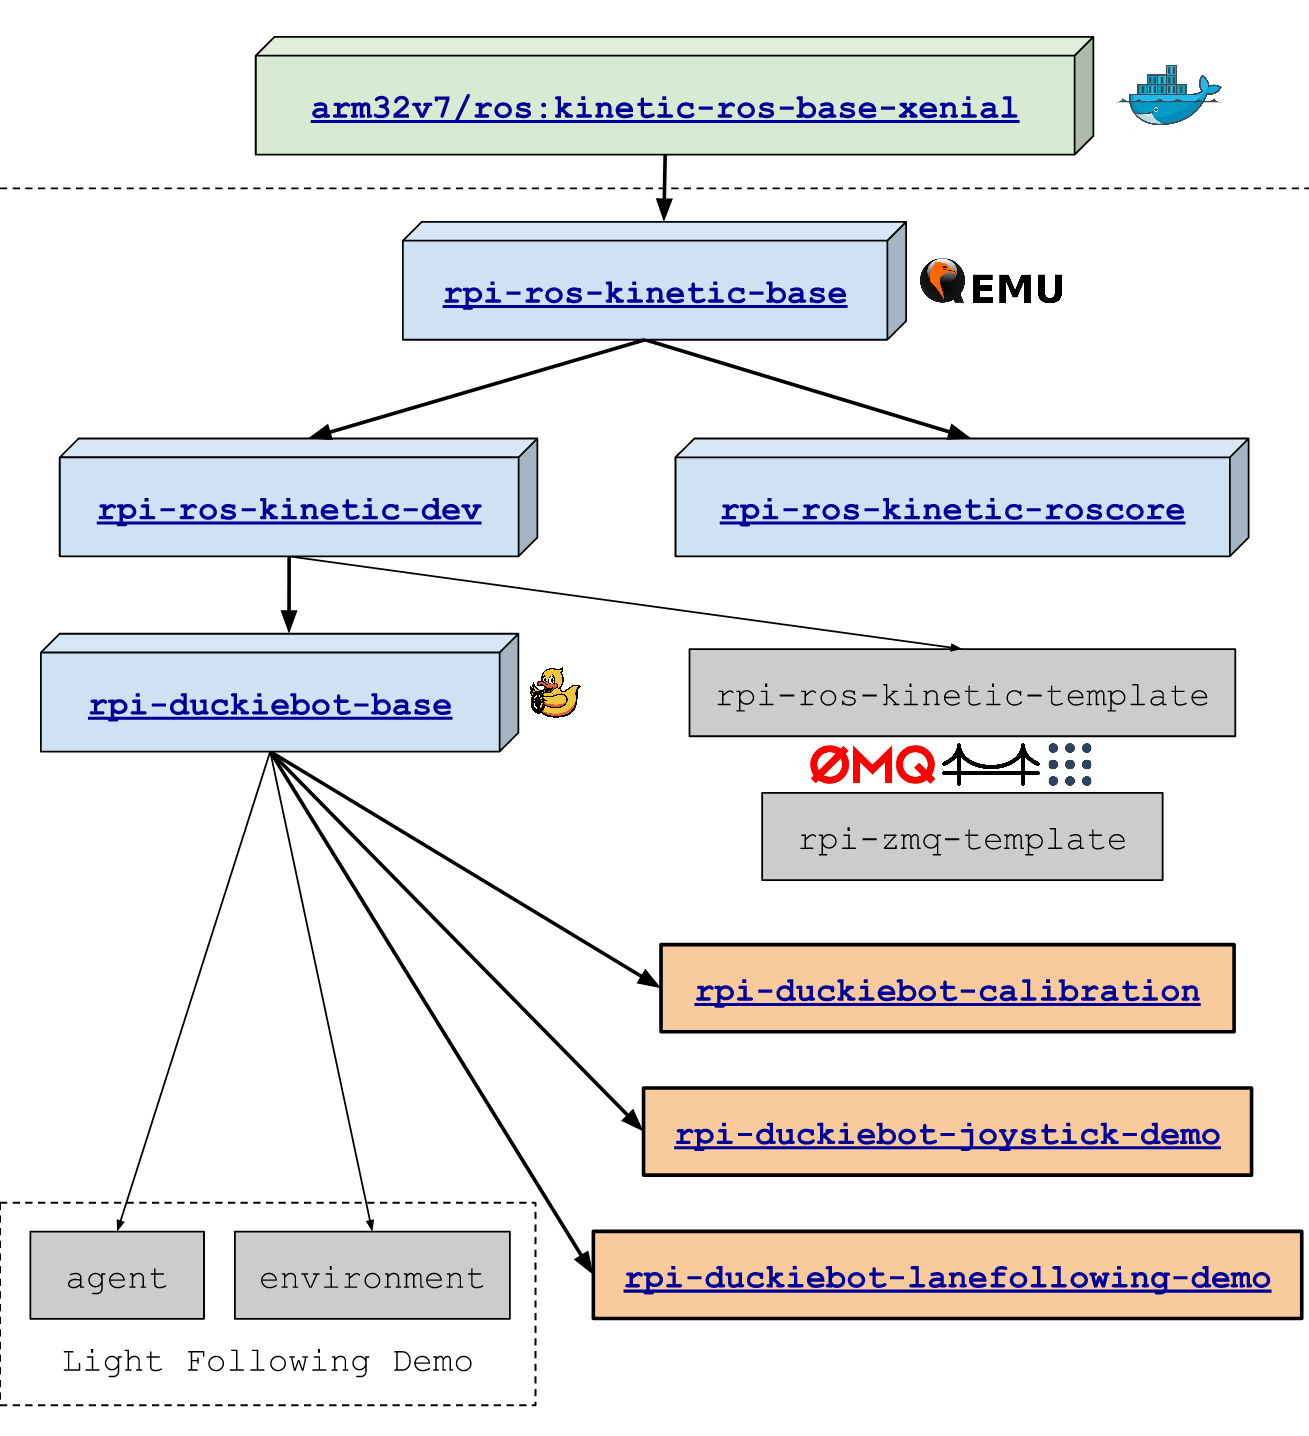
\includegraphics[width=0.80\textwidth]{../figures/image_provenance.png}
\caption{Early prototype of the Docker image hierarchy. Chaining unversioned autobuilds without disciplined unit testing creates a potential domino effect which allows breaking changes to propagate downstream, resulting in a cascade of silent failures.}
\label{fig:early_prototype}
\end{figure}

The root cause of this friction was a product of imprecise versioning and over-automation. As version tags were initially omitted, all images were pulled and built from the latest commit on the mainline development branch. The auto-build feature of the CI server caused upstream modifications to cascade to downstream images. Our short-term solution was to disable auto-building, and push local builds to the server manually, however fixing it required us to rethink the role of versioning and testing Docker builds in the CI toolchain.

\begin{figure}

\includegraphics[width=0.40\textwidth]{../figures/aido_logo.png}
\caption{The \href{https://www.duckietown.org/research/ai-driving-olympics}{AI Driving Olympics}, a primary use case for the system described above.}
\label{fig:aido_logo}
\end{figure}

A more stable solution is to store all sources on the local development environment and rebuild the image only when its upstream dependencies change. The image only contains its compiled upstream dependencies and is only paired with source code at runtime.

One of the primary use cases for the Duckietown container infrastructure is a biannual autonomous robotics competition called the AI Driving Olympics~\citep{aido2018} (AIDO). To participate, competitors must submit a Docker image (various templates are provided for \href{https://github.com/duckietown/challenge-aido_LF-baseline-RL-sim-pytorch}{reinforcement learning}, \href{https://github.com/duckietown/challenge-aido_LF-baseline-IL-logs-tensorflow}{imitation learning} and \href{https://github.com/duckietown/challenge-aido_LF-template-ros}{classical robotics}). The submitted image, together with a Git repository and a commit hash, constitutes an AIDO submission. The submission is retrieved by the organizers and evaluated on a random map in Duckietown's \href{https://github.com/duckietown/gym-duckietown}{simulator}~\citep{gym_duckietown}. This evaluation produces a numerical score in several categories. Valid submissions may also be run on a physical \textit{robotarium}. The highest ranking submissions are evaluated in a final round at NeurIPS and ICRA.

\subsection{Remarks on security}

An unfortunate technical shortcoming of the Docker system is its reliance on superuser privileges. While Docker takes a variety of preventative measures to ensure container inhabitants cannot gain escalated privileges, numerous breakout attacks have been discovered~\citep{martin2018docker} in the wild. Any process which can circumvent container security gains unfettered access to the host OS, making Docker especially unsuitable for deployment on cloud, grid, and cluster computing environments.

Furthermore, Docker provides a mechanism to bypass its own security measures, allowing container applications to run as if they were root processes on the host OS: the \href{https://docs.docker.com/engine/reference/run/#security-configuration}{\inline{-{}-privileged} flag}. This feature, alongside the fact that most Docker users are unqualified to audit upstream images, which are liable to include packages of dubious provenance~\citep{martin2018docker}, makes Docker particularly unsuitable for shared-computing environments.

Docker's unnecessarily high privileges and susceptibility for misuse are serious issues. While operator error may be partly at fault, these vulnerabilities are primarily the result of poor implementation choices. Docker's flagrant violation of the principle of least privilege~\citep{saltzer1975protection} effectively compromises the entire Linux security model.

To address these issues, various container platforms, including \href{https://docs.nersc.gov/programming/shifter/overview/}{Shifter}~\citep{gerhardt2017shifter} and \href{https://sylabs.io/docs/}{Singularity}~\citep{kurtzer2017singularity}, have emerged and gained traction in the scientific computing community, owing to their lower privileges and compatibility with legacy Linux distributions used by many academic computing environments. Since then, Docker has also introduced a \href{https://engineering.docker.com/2019/02/experimenting-with-rootless-docker/}{rootless mode}, but it remains experimental at the time of writing this thesis.

\section{Conclusion}

In this chapter, we have taken a guided tour through the process of containerization and demonstrated the effectiveness of containers for building reproducible robotics software -- a key step in the broader quest for experimental reproducibility. We propose a set of best practices and lessons learned during the design, development and deployment of Docker containers for the Duckietown~\citep{paull2017duckietown} platform. We also recommend a number of tools and techniques for software reproducibility, a key component in the broader quest for reproducible research. The author wishes to thank Rusi Hristov for his invaluable technical assistance during the initial stages of this project and Florian Golemo for architectural planning and assistance. For more information about the Duckietown platform and reproducible software development using Docker, please visit: \url{https://docs.duckietown.org}